\documentclass[11pt,a4paper]{article}
\usepackage[utf8]{inputenc}
\usepackage[T1]{fontenc}
\usepackage{lmodern}
\usepackage[margin=2.3cm]{geometry}
\usepackage{amsmath}
\usepackage{booktabs}
\usepackage{graphicx}
\usepackage{float}
\usepackage{xcolor}
\usepackage{listings}
\usepackage{caption}
\usepackage{enumitem}
\usepackage{needspace}
\usepackage[hidelinks]{hyperref}

\definecolor{fundo}{HTML}{F6F6F4}
\definecolor{chave}{HTML}{1C5CAB}
\definecolor{coment}{HTML}{6B6B66}
\lstset{
  language=C, basicstyle=\ttfamily\small, backgroundcolor=\color{fundo},
  keywordstyle=\color{chave}\bfseries, commentstyle=\color{coment},
  frame=single, rulecolor=\color{fundo}, framesep=4pt, xleftmargin=6pt, xrightmargin=6pt,
  columns=fullflexible, keepspaces=true, showstringspaces=false,
  morekeywords={pragma,omp,parallel,for,reduction,schedule,static,min,max},
  literate={ã}{{\~a}}1 {ç}{{\c c}}1 {é}{{\'e}}1 {á}{{\'a}}1
}
\setlist{itemsep=2pt, topsep=4pt}
\captionsetup{font=small, labelfont=bf}

\title{\textbf{Exercício Final: Análise de Dados com OpenMP}\\[4pt]
\large Coeficiente de variação para dados agrupados em classes}
\author{Yuri Victor de Oliveira e Silva\\
\small Ciência da Computação -- IESB \quad|\quad Programação Paralela -- Prof.\ Rodrigo}
\date{Novembro de 2026}

\begin{document}
\renewcommand{\tablename}{Tabela}
\renewcommand{\figurename}{Figura}
\maketitle

\section{Objetivo e visão geral}

O programa \texttt{coef\_variacao.c} lê a estatura (cm) e o peso (kg) de 1000 pessoas,
agrupa cada variável em intervalos de classe (8\,cm para estatura e 4\,kg para peso) e calcula,
para cada uma, a média ponderada, o desvio padrão populacional e o coeficiente de variação (CV).
Os laços de cálculo foram paralelizados com OpenMP.

Para comparar as versões de forma justa, \textbf{o mesmo arquivo-fonte} gera dois executáveis:
\begin{itemize}
  \item \texttt{cv\_seq}: compilado \emph{sem} \texttt{-fopenmp}. O compilador ignora todas as diretivas
        \texttt{\#pragma omp} e o código roda sequencialmente;
  \item \texttt{cv\_par}: compilado \emph{com} \texttt{-fopenmp}. As diretivas são ativadas.
\end{itemize}
Assim, o algoritmo é idêntico nas duas versões e a diferença de tempo vem apenas do paralelismo.

\section{Dados de entrada}

O enunciado não traz o arquivo de dados. Por isso foi gerada uma base de 1000 pessoas com o script
\texttt{gerar\_dados.py} (semente fixa 2026, portanto reprodutível). As estaturas seguem distribuições normais
por sexo (média de 175\,cm e 162\,cm), e o peso é obtido a partir de um IMC sorteado. O arquivo
\texttt{dados.txt} segue o formato pedido: uma pessoa por linha, com estatura e peso separados por espaço.
O programa aceita qualquer arquivo nesse formato. Basta executar \texttt{./cv\_par arquivo.txt}.
A leitura também aceita vírgula decimal (\texttt{172,4 81,8}), separadores \texttt{;}, \texttt{,} ou tabulação,
quebra de linha do Windows, linhas em branco e uma linha de cabeçalho. Linhas inválidas (texto, valores
negativos ou nulos, colunas a mais) são descartadas com um aviso informando quantas foram e onde está a primeira,
para que um problema no arquivo não altere o resultado sem que o usuário perceba.

\section{Construção das classes e fórmulas}

Para uma amplitude de classe $h$, o limite inferior da primeira classe é o maior múltiplo de $h$
que não ultrapassa o menor valor observado, e o número de classes $k$ é o necessário para cobrir o maior valor:
\[
  L_1 = \left\lfloor \frac{\min(x)}{h} \right\rfloor h, \qquad
  k = \left\lfloor \frac{\max(x) - L_1}{h} \right\rfloor + 1 .
\]
As classes são fechadas à esquerda e abertas à direita ($L_i \vdash L_i + h$). Um valor $v$ pertence à classe
$\lfloor (v - L_1)/h \rfloor$, e o ponto médio da classe $i$ é $x_i = L_1 + (i - \tfrac12)h$.
Em seguida são aplicadas as fórmulas do enunciado:
\[
  \mu = \frac{\sum_{i=1}^{k} x_i f_i}{N}, \qquad
  \sigma = \sqrt{\frac{\sum_{i=1}^{k} f_i (x_i - \mu)^2}{N}}, \qquad
  CV = \frac{\sigma}{\mu}\times 100\% .
\]

\section{O que foi paralelizado e por quê}

A Tabela~\ref{tab:lacos} resume os laços do programa. A ideia central é: \textbf{cada laço que acumula um valor
(soma, contagem, mínimo, máximo) usa a cláusula \texttt{reduction}}. Cada thread acumula numa cópia privada da
variável, e o OpenMP combina as cópias no final. Isso elimina a condição de corrida (duas threads
escrevendo na mesma variável ao mesmo tempo) sem precisar de \texttt{critical} ou \texttt{atomic}, que
serializariam o acesso e destruiriam o ganho.

\begin{table}[H]
\centering
\footnotesize
\caption{Laços do programa, custo e diretiva OpenMP usada.}
\label{tab:lacos}
\begin{tabular}{@{}lcll@{}}
\toprule
Função & Custo & Cláusulas do \texttt{parallel for} & Motivo \\
\midrule
\texttt{calcular\_extremos} & $O(N)$ & \texttt{reduction(min:mn) reduction(max:mx)} & limites das classes \\
\texttt{contar\_frequencias} & $O(N)$ & \texttt{reduction(+:freq[:k])} & frequências $f_i$ \\
\texttt{calcular\_media\_agrupada} & $O(k)$ & \texttt{reduction(+:soma\_xf, soma\_f)} & média $\mu$ \\
\texttt{calcular\_desvio\_agrupado} & $O(k)$ & \texttt{reduction(+:soma)} & desvio $\sigma$ \\
\texttt{calcular\_estatisticas\_brutas} & $O(N)$ & \texttt{reduction(+:soma)}; \texttt{reduction(+:soma\_quad)} & conferência \\
\bottomrule
\end{tabular}
\end{table}

\paragraph{Contagem das frequências (o laço mais importante).}
É o laço que percorre as $N$ pessoas. Se várias threads fizessem \texttt{freq[classe]++} no mesmo vetor
compartilhado, incrementos se perderiam. A redução de vetor (\texttt{freq[:k]}, disponível desde o OpenMP 4.5)
dá a cada thread um histograma privado de $k$ posições, que é somado ao final:
\begin{lstlisting}
#pragma omp parallel for reduction(+:freq[:k]) schedule(static)
for (long i = 0; i < n; i++) {
    int classe = (int)((v[i] - li) / h);
    if (classe >= k) classe = k - 1;
    freq[classe]++;
}
\end{lstlisting}

\paragraph{Soma, média e desvio padrão.}
São os laços pedidos explicitamente no enunciado. Para os dados agrupados, eles percorrem as $k$ classes:
\begin{lstlisting}
#pragma omp parallel for reduction(+:soma_xf, soma_f) schedule(static)
for (int i = 0; i < d->k; i++) {
    soma_xf += ponto_medio(d, i) * d->freq[i];
    soma_f  += d->freq[i];
}
...
#pragma omp parallel for reduction(+:soma) schedule(static)
for (int i = 0; i < d->k; i++) {
    double desvio = ponto_medio(d, i) - mu;
    soma += d->freq[i] * desvio * desvio;
}
\end{lstlisting}
Há uma ressalva importante: aqui $k$ vale apenas 9 (estatura) e 25 (peso). Com tão poucas iterações, o
custo de criar e sincronizar as threads é maior que o próprio cálculo, então esses dois laços não ficam
mais rápidos. Eles foram paralelizados porque o enunciado pede. O trabalho pesado, que cresce com $N$, está nos
laços $O(N)$ (extremos, frequências e estatísticas brutas). É neles que o paralelismo traz ganho real.

\paragraph{Escalonamento.} Usou-se \texttt{schedule(static)} em todos os laços, porque cada iteração tem o mesmo
custo. Dividir as iterações em blocos contíguos iguais tem o menor overhead e mantém cada thread lendo uma faixa
contínua da memória, o que aproveita bem o cache.

\paragraph{O que \emph{não} foi paralelizado.}
\begin{itemize}
  \item \textbf{Leitura do arquivo}: o arquivo é lido linha a linha (\texttt{fgets} e \texttt{sscanf}). Ler um único arquivo texto
        com várias threads não traz ganho e complicaria o código. A leitura também fica fora da medição de tempo
        (com $N=1000$, ela leva cerca de 0,5\,ms, muito mais que o cálculo).
  \item \textbf{Montagem das classes}: são poucas operações aritméticas, com custo $O(1)$.
  \item \textbf{Impressão das tabelas}: é saída de texto, com custo $O(k)$ e ordem fixa.
\end{itemize}

\section{Resultados}

As versões sequencial e paralela (com 1, 2 e 4 threads) produziram exatamente os mesmos valores.
As tabelas de distribuição de frequências estão abaixo, e a Figura~\ref{fig:hist} mostra os histogramas.

\begin{table}[H]
\centering
\small
\caption{Distribuição de frequências da estatura (amplitude $h = 8$\,cm, $k = 9$ classes).}
\begin{tabular}{@{}clrrrr@{}}
\toprule
$i$ & Classe (cm) & $x_i$ & $f_i$ & $x_i f_i$ & $f_i (x_i - \mu)^2$ \\
\midrule
1 & $136 \vdash 144$ & 140 & 2 & 280 & 1.540,35 \\
2 & $144 \vdash 152$ & 148 & 34 & 5.032 & 13.264,81 \\
3 & $152 \vdash 160$ & 156 & 181 & 28.236 & 24.997,82 \\
4 & $160 \vdash 168$ & 164 & 301 & 49.364 & 4.237,33 \\
5 & $168 \vdash 176$ & 172 & 283 & 48.676 & 5.106,88 \\
6 & $176 \vdash 184$ & 180 & 159 & 28.620 & 23.852,15 \\
7 & $184 \vdash 192$ & 188 & 38 & 7.144 & 15.579,30 \\
8 & $192 \vdash 200$ & 196 & 1 & 196 & 797,95 \\
9 & $200 \vdash 208$ & 204 & 1 & 204 & 1.313,92 \\
\midrule
 & \textbf{Total} & & \textbf{1000} & \textbf{167.752} & \textbf{90.690,50} \\
\bottomrule

\end{tabular}
\end{table}

\begin{align*}
\mu_{\text{est}} &= \frac{167\,752}{1000} = 167{,}752\ \text{cm}, \qquad
\sigma_{\text{est}} = \sqrt{\frac{90\,690{,}50}{1000}} = 9{,}5232\ \text{cm},\\
CV_{\text{est}} &= \frac{9{,}5232}{167{,}752}\times 100\% = \mathbf{5{,}68\%}
\end{align*}

\begin{figure}[H]
\centering
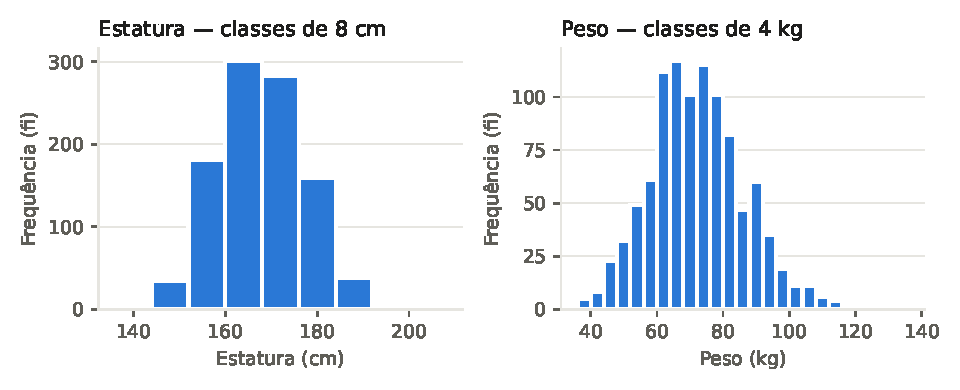
\includegraphics[width=0.95\textwidth]{fig_histogramas.pdf}
\caption{Histogramas das classes usadas no cálculo.}
\label{fig:hist}
\end{figure}

\begin{table}[H]
\centering
\footnotesize
\renewcommand{\arraystretch}{0.92}
\caption{Distribuição de frequências do peso (amplitude $h = 4$\,kg, $k = 25$ classes).}
\begin{tabular}{@{}clrrrr@{}}
\toprule
$i$ & Classe (kg) & $x_i$ & $f_i$ & $x_i f_i$ & $f_i (x_i - \mu)^2$ \\
\midrule
1 & $36 \vdash 40$ & 38 & 5 & 190 & 5.898,93 \\
2 & $40 \vdash 44$ & 42 & 8 & 336 & 7.368,01 \\
3 & $44 \vdash 48$ & 46 & 23 & 1.058 & 15.966,99 \\
4 & $48 \vdash 52$ & 50 & 32 & 1.600 & 15.981,86 \\
5 & $52 \vdash 56$ & 54 & 49 & 2.646 & 16.495,81 \\
6 & $56 \vdash 60$ & 58 & 61 & 3.538 & 12.557,77 \\
7 & $60 \vdash 64$ & 62 & 112 & 6.944 & 11.993,08 \\
8 & $64 \vdash 68$ & 66 & 117 & 7.722 & 4.714,76 \\
9 & $68 \vdash 72$ & 70 & 101 & 7.070 & 556,82 \\
10 & $72 \vdash 76$ & 74 & 115 & 8.510 & 313,85 \\
11 & $76 \vdash 80$ & 78 & 101 & 7.878 & 3.226,46 \\
12 & $80 \vdash 84$ & 82 & 82 & 6.724 & 7.639,21 \\
13 & $84 \vdash 88$ & 86 & 47 & 4.042 & 8.759,72 \\
14 & $88 \vdash 92$ & 90 & 60 & 5.400 & 18.695,59 \\
15 & $92 \vdash 96$ & 94 & 35 & 3.290 & 16.408,32 \\
16 & $96 \vdash 100$ & 98 & 19 & 1.862 & 12.502,48 \\
17 & $100 \vdash 104$ & 102 & 11 & 1.122 & 9.671,65 \\
18 & $104 \vdash 108$ & 106 & 11 & 1.166 & 12.457,03 \\
19 & $108 \vdash 112$ & 110 & 6 & 660 & 8.506,04 \\
20 & $112 \vdash 116$ & 114 & 4 & 456 & 6.939,56 \\
21 & $116 \vdash 120$ & 118 & 0 & 0 & 0,00 \\
22 & $120 \vdash 124$ & 122 & 0 & 0 & 0,00 \\
23 & $124 \vdash 128$ & 126 & 0 & 0 & 0,00 \\
24 & $128 \vdash 132$ & 130 & 0 & 0 & 0,00 \\
25 & $132 \vdash 136$ & 134 & 1 & 134 & 3.800,97 \\
\midrule
 & \textbf{Total} & & \textbf{1000} & \textbf{72.348} & \textbf{200.454,90} \\
\bottomrule

\end{tabular}
\end{table}

\begin{align*}
\mu_{\text{peso}} &= \frac{72\,348}{1000} = 72{,}348\ \text{kg}, \qquad
\sigma_{\text{peso}} = \sqrt{\frac{200\,454{,}90}{1000}} = 14{,}1582\ \text{kg},\\
CV_{\text{peso}} &= \frac{14{,}1582}{72{,}348}\times 100\% = \mathbf{19{,}57\%}
\end{align*}


\begin{table}[H]
\centering
\small
\caption{Resumo dos resultados e conferência com os dados brutos (não agrupados).}
\label{tab:resumo}
\begin{tabular}{@{}lrrrr@{}}
\toprule
Variável & $\mu$ & $\sigma$ & \textbf{CV (agrupado)} & CV (dados brutos) \\
\midrule
Estatura (cm) & 167,752 & 9,5232 & \textbf{5,68\%} & 5,51\% \\
Peso (kg)     & 72,348  & 14,1582 & \textbf{19,57\%} & 19,53\% \\
\bottomrule
\end{tabular}
\end{table}

\paragraph{Interpretação.} O peso tem dispersão relativa cerca de 3,4 vezes maior que a estatura. Pela
classificação usual (CV $\le 15\%$: baixa dispersão; $15\%$ a $30\%$: média; $> 30\%$: alta), a estatura é
\textbf{homogênea}, com baixa dispersão, e o peso tem \textbf{dispersão média}. É justamente para essa comparação
que o CV existe: como ele é adimensional, permite comparar variáveis medidas em unidades diferentes (cm e kg).

\paragraph{Conferência.} Os valores agrupados foram conferidos com um script Python independente (mesmas
frequências, médias e desvios). Também foram comparados com as estatísticas calculadas sobre os dados brutos
(Tabela~\ref{tab:resumo}). A pequena diferença é esperada: no agrupamento, cada pessoa é representada pelo
ponto médio da sua classe, e classes largas, como as de 8\,cm, tendem a inflar levemente o desvio padrão.

\section{Análise de desempenho}

\paragraph{Ambiente e metodologia.} Intel Xeon 2,10\,GHz com \textbf{2 núcleos físicos} (sem hyper-threading),
L2 de 2\,MiB por núcleo, Ubuntu 24.04, GCC 13.3 com \texttt{-O2}, \texttt{OMP\_PROC\_BIND=close}. Mede-se apenas a
fase de cálculo das duas variáveis (extremos, classes, frequências, média, desvio, CV e estatísticas brutas),
com \texttt{clock\_gettime(CLOCK\_MONOTONIC)}. A leitura do arquivo fica de fora. Cada configuração foi executada
muitas vezes (5000 repetições para $N = 1000$ e 10 para $N = 2\times10^7$), e o script \texttt{benchmark.sh} foi
rodado 3 vezes; o valor reportado é a mediana. Além do arquivo de 1000 pessoas, o programa gera em memória bases
sintéticas maiores (\texttt{--sintetico N}) para observar como o ganho escala com o tamanho da entrada.
Speedup: $S = T_{\text{seq}}/T_{\text{par}}$. Eficiência: $E = S/p$, onde $p$ é o número de threads.

\begin{table}[H]
\centering
\small
\caption{Tempo de cálculo (ms, mediana), speedup e eficiência.}
\label{tab:desemp}
\begin{tabular}{@{}rrrrrrrr@{}}
\toprule
 & \textbf{Sequencial} & \multicolumn{3}{c}{\textbf{Paralela, 2 threads}} & \multicolumn{3}{c}{\textbf{Paralela, 4 threads}} \\
\cmidrule(lr){2-2}\cmidrule(lr){3-5}\cmidrule(l){6-8}
$N$ & tempo & tempo & $S$ & $E$ & tempo & $S$ & $E$ \\
\midrule
1.000 & 0,0078 & 0,0218 & 0,36 & 18\% & 0,4073 & 0,02 & 0\% \\
10.000 & 0,0753 & 0,0602 & 1,25 & 63\% & 0,4882 & 0,15 & 4\% \\
100.000 & 0,8779 & 0,4220 & 2,08 & 104\% & 0,9100 & 0,96 & 24\% \\
1.000.000 & 8,6705 & 4,9590 & 1,75 & 87\% & 5,5805 & 1,55 & 39\% \\
10.000.000 & 177,9144 & 95,7639 & 1,86 & 93\% & 96,9843 & 1,83 & 46\% \\
20.000.000 & 355,0490 & 188,4934 & 1,88 & 94\% & 191,6658 & 1,85 & 46\% \\
\bottomrule

\end{tabular}
\end{table}

\begin{figure}[tbp]
\centering
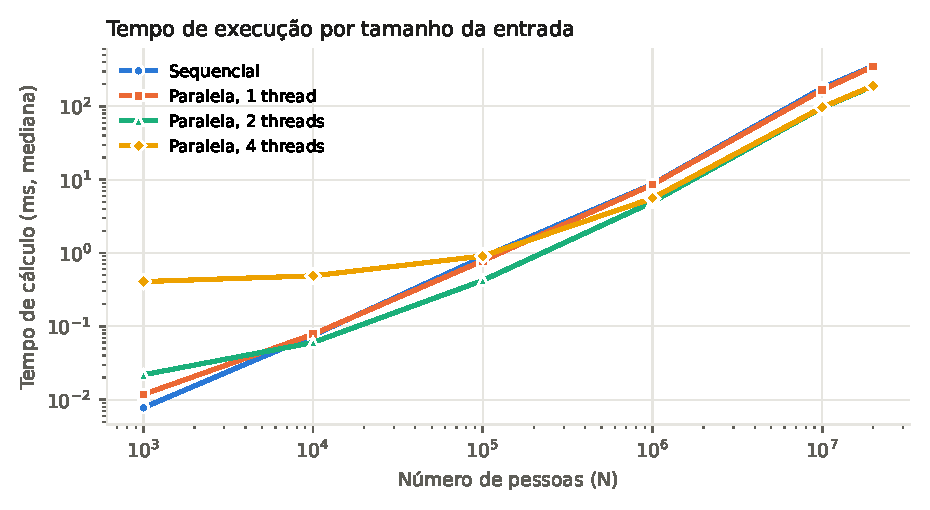
\includegraphics[width=0.8\textwidth]{fig_tempo.pdf}
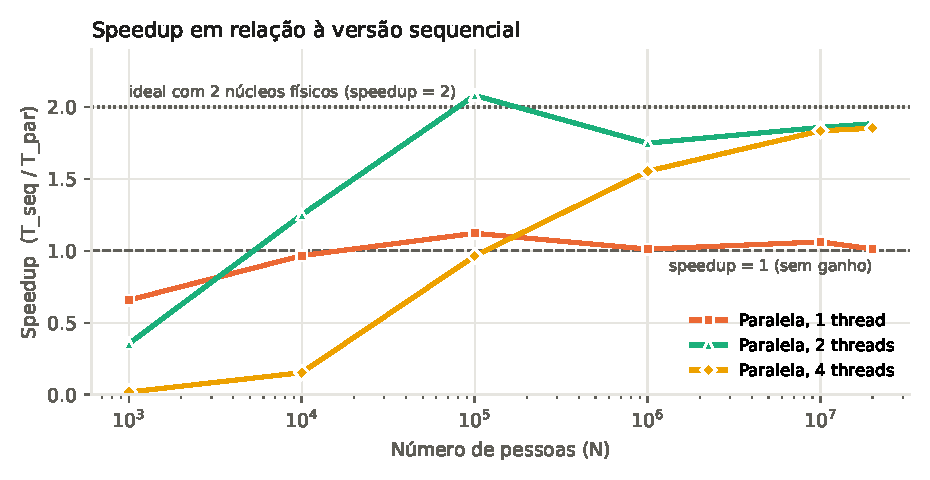
\includegraphics[width=0.8\textwidth]{fig_speedup.pdf}
\caption{Tempo de execução (escala log-log) e speedup em relação à versão sequencial.}
\label{fig:desemp}
\end{figure}

\paragraph{O caso pedido ($N = 1000$): a versão paralela é mais lenta.} O cálculo sequencial leva cerca de
\textbf{7,8\,$\mu$s}, contra \textbf{21,8\,$\mu$s} com 2 threads ($S \approx 0{,}36$). Cada execução abre 12 regiões
paralelas (6 por variável), e cada uma tem um custo fixo de distribuir o trabalho e sincronizar as threads na barreira
final, da ordem de microssegundos. Com 1000 pessoas, cada thread faz poucas centenas de operações por laço, então
esse custo fixo domina. Pela Lei de Amdahl e pelo próprio overhead do OpenMP, paralelizar um problema desse tamanho
não compensa. A curva ``Paralela, 1 thread'' da Figura~\ref{fig:desemp} confirma isso: ativar o OpenMP sem dividir o trabalho
já custa cerca de 4\,$\mu$s a mais.

\paragraph{A partir de $N \approx 10^4$ o paralelismo compensa.} Com $10^4$ pessoas o ganho começa
($S \approx 1{,}25$). De $10^6$ em diante, o speedup estabiliza entre 1,75 e 1,88 com 2 threads, ou seja,
eficiência de 87\% a 94\%, próxima do ideal de 2 numa máquina com 2 núcleos. O que falta para chegar a 2 vem das
partes sequenciais (montagem das classes, laços $O(k)$, alocação) e da banda de memória: com bases grandes, os
laços apenas leem vetores e fazem pouca conta, então o limite passa a ser a velocidade da RAM. Em $N = 10^5$
apareceu um speedup um pouco acima de 2 ($S \approx 2{,}08$), que se repetiu nas 3 rodadas. A explicação mais
provável é efeito de cache: dividindo os dados, cada núcleo trabalha com metade deles no seu cache L2 privado,
e o conjunto inteiro passa a ser servido por dois caches em vez de um.

\paragraph{4 threads em 2 núcleos não ajudam.} Com mais threads que núcleos, as threads disputam o mesmo
processador. Para entradas pequenas, o custo de troca de contexto e de espera nas barreiras é alto
(0,41\,ms para $N=1000$, mais de 50 vezes o sequencial). Para entradas grandes, o resultado só empata com o
de 2 threads. Numa máquina com mais núcleos (por exemplo, 6 núcleos e 12 threads), o mesmo
\texttt{benchmark.sh} deve mostrar speedups maiores para $N$ grande. Basta ajustar \texttt{THREADS="1 2 4 6 12"}.

\section{Testes e validação}

O script \texttt{testes/rodar\_testes.sh} executa 32 verificações automáticas, e todas passaram:
\begin{itemize}
  \item \textbf{Compilação estrita}: as duas versões compilam sem avisos com \texttt{-Wall -Wextra -Wpedantic -Werror}.
  \item \textbf{Conferência independente}: um script Python recalcula limites, classes, $f_i$, $\mu$, $\sigma$ e CV com
        aritmética exata (frações) e atribui as classes por comparação com os limites, não por divisão como o
        programa em C. Os valores bateram em todas as casas impressas. Um exemplo pequeno com 4 pessoas, com valores
        exatamente sobre os limites das classes, foi calculado à mão e também bateu (CV de 3,6262\% e 7,9253\%).
  \item \textbf{Sequencial $\times$ paralela}: a saída é idêntica com 1, 2, 3, 4, 6, 8 e 12 threads, com
        \texttt{-O0} e \texttt{-O3}, com o \texttt{clang} (versão sequencial) e com
        bases de até $10^7$ pessoas.
  \item \textbf{Casos de borda}: uma única pessoa, valores todos iguais (CV $= 0$), cabeçalho, vírgula decimal,
        separadores variados, linhas inválidas, arquivo vazio, arquivo inexistente e valores absurdos (que gerariam
        milhões de classes). Os três últimos encerram o programa com uma mensagem de erro clara.
  \item \textbf{Memória}: AddressSanitizer, UndefinedBehaviorSanitizer e Valgrind não acusaram nenhum acesso
        inválido, vazamento ou comportamento indefinido.
  \item \textbf{Condição de corrida}: o ThreadSanitizer, combinado com o Archer (ferramenta do LLVM que informa ao
        TSan a sincronização do OpenMP), não encontrou nenhuma corrida. Para garantir que o teste detecta o problema,
        foi feita uma cópia do código sem o \texttt{reduction} na contagem das frequências: o TSan apontou a corrida
        na linha do \texttt{freq[classe]++}, e com 8 threads e $10^7$ pessoas a contagem perdeu de 33\% a 40\% das
        pessoas. Isso mostra, na prática, por que a redução é necessária.
\end{itemize}

\needspace{10\baselineskip}
\section{Como compilar e executar}

\begin{lstlisting}[language=bash]
make                       # gera cv_seq (sequencial) e cv_par (OpenMP)
./cv_seq dados.txt         # tabelas, CVs e tempo da versao sequencial
OMP_NUM_THREADS=2 ./cv_par dados.txt
./cv_par --sintetico 10000000 10   # base sintetica de 10 milhoes de pessoas
./benchmark.sh             # gera resultados.csv com todos os tempos
./testes/rodar_testes.sh   # executa as 32 verificacoes automaticas
\end{lstlisting}

\section{Conclusão}

O programa calcula corretamente os coeficientes de variação para dados agrupados: \textbf{CV da estatura
$= 5{,}68\%$} (baixa dispersão) e \textbf{CV do peso $= 19{,}57\%$} (dispersão média). O OpenMP foi aplicado
com cláusulas \texttt{reduction} em todos os laços de acumulação, o que garante resultados corretos e idênticos
aos da versão sequencial. A análise de desempenho mostrou que, para as 1000 pessoas do enunciado, o overhead
do paralelismo supera o ganho. Para entradas a partir de dezenas de milhares de registros, porém, a versão
paralela fica quase duas vezes mais rápida em 2 núcleos, com eficiência próxima de 90\%. Ou seja, paralelizar
vale a pena quando há trabalho suficiente para dividir entre as threads.

\end{document}
